\chapter{Supplementary Materials}
\label{appendix:supplementary-materials}

% Appendix figures and tables share one continuous display-item counter.
\makeatletter
\let\c@table\c@figure
\let\thetable\thefigure
\makeatother

\section{Processing-Demand Estimator Sensitivity}
\label{appendix:pdb-sensitivity}

\begin{table}[H]
\centering
\caption{Reproducibility and cross-estimator sensitivity of the frozen PDB annotations.}
\label{tab:appendix-pdb-sensitivity}
\small
\setlength{\tabcolsep}{8pt}
\renewcommand{\arraystretch}{1.15}
\begin{tabular*}{0.82\textwidth}{@{\extracolsep{\fill}}>{\raggedright\arraybackslash}p{0.58\textwidth}r@{}}
\toprule
\textbf{Validation metric} & \textbf{Result} \\
\midrule
Maximum frozen-value reproduction error & 0.000349 bits \\
Maximum range across ten repeated calculations & 0 bits \\
Cross-estimator Spearman $\rho$ & 0.864 \\
Lesson-stratified bootstrap 95\% CI & $[0.782,0.917]$ \\
Lesson-level $\rho$ range & $0.782$--$0.952$ \\
Low-tail Jaccard similarity & 0.615 \\
High-tail Jaccard similarity & 0.448 \\
Low/Middle/High agreement & 68.7\% \\
Unweighted Cohen's $\kappa$ & 0.501 \\
Low--High extreme flips & 0 \\
\bottomrule
\end{tabular*}
\end{table}

\section{Human-Scoring Disagreement Audit}
\label{appendix:human-disagreement-audit}

\begin{table}[H]
\centering
\caption{Structured audit of human--human scoring disagreements.}
\label{tab:appendix-human-disagreement-audit}
\scriptsize
\setlength{\tabcolsep}{2pt}
\renewcommand{\arraystretch}{1.15}
\begin{tabular*}{\textwidth}{@{\extracolsep{\fill}}>{\raggedright\arraybackslash}p{0.09\textwidth}>{\raggedright\arraybackslash}p{0.07\textwidth}>{\raggedright\arraybackslash}p{0.08\textwidth}>{\raggedright\arraybackslash}p{0.08\textwidth}>{\raggedright\arraybackslash}p{0.20\textwidth}>{\raggedright\arraybackslash}p{0.39\textwidth}@{}}
\toprule
\textbf{Question} & \makecell{\textbf{Crite-}\\\textbf{rion}} & \textbf{Human 1} & \textbf{Human 2} & \textbf{Disagreement category} & \textbf{Audit summary} \\
\midrule
\texttt{L01\_QC03} & \texttt{C1} & Absent & Correct & Required-component completeness & The answer described the financial system and three participant groups but did not explicitly include businesses. \\
\texttt{L01\_QC08} & \texttt{C2} & Correct & Absent & Conceptual equivalence & The disagreement concerned whether asset allocation across classes sufficiently expresses diversification. \\
\texttt{L03\_QC07} & \texttt{C1} & Absent & Correct & Implicit contrast & The answer contrasted raw data with meaningful information without directly stating ``not merely collecting more data.'' \\
\texttt{L04\_QC02} & \texttt{C1} & Absent & Correct & Category--instance mapping & The answer named CFO and related positions without directly using the broader role label ``financial manager.'' \\
\texttt{L04\_QC09} & \texttt{C3} & Correct & Absent & Distributed relational evidence & Technical solutions, IT teams, and modelling contrasts appeared across the answer, but the target relation was not expressed as one explicit proposition. \\
\bottomrule
\end{tabular*}

\vspace{2pt}
\parbox{\textwidth}{\footnotesize\textit{Note.} This audit characterises the semantic boundary underlying each original disagreement. It does not overwrite either rater's independent label or construct a forced consensus reference.}
\end{table}

\section{LLM Judge Prompt}
\label{appendix:llm-judge-prompt}

\begin{figure}[H]
    \centering
    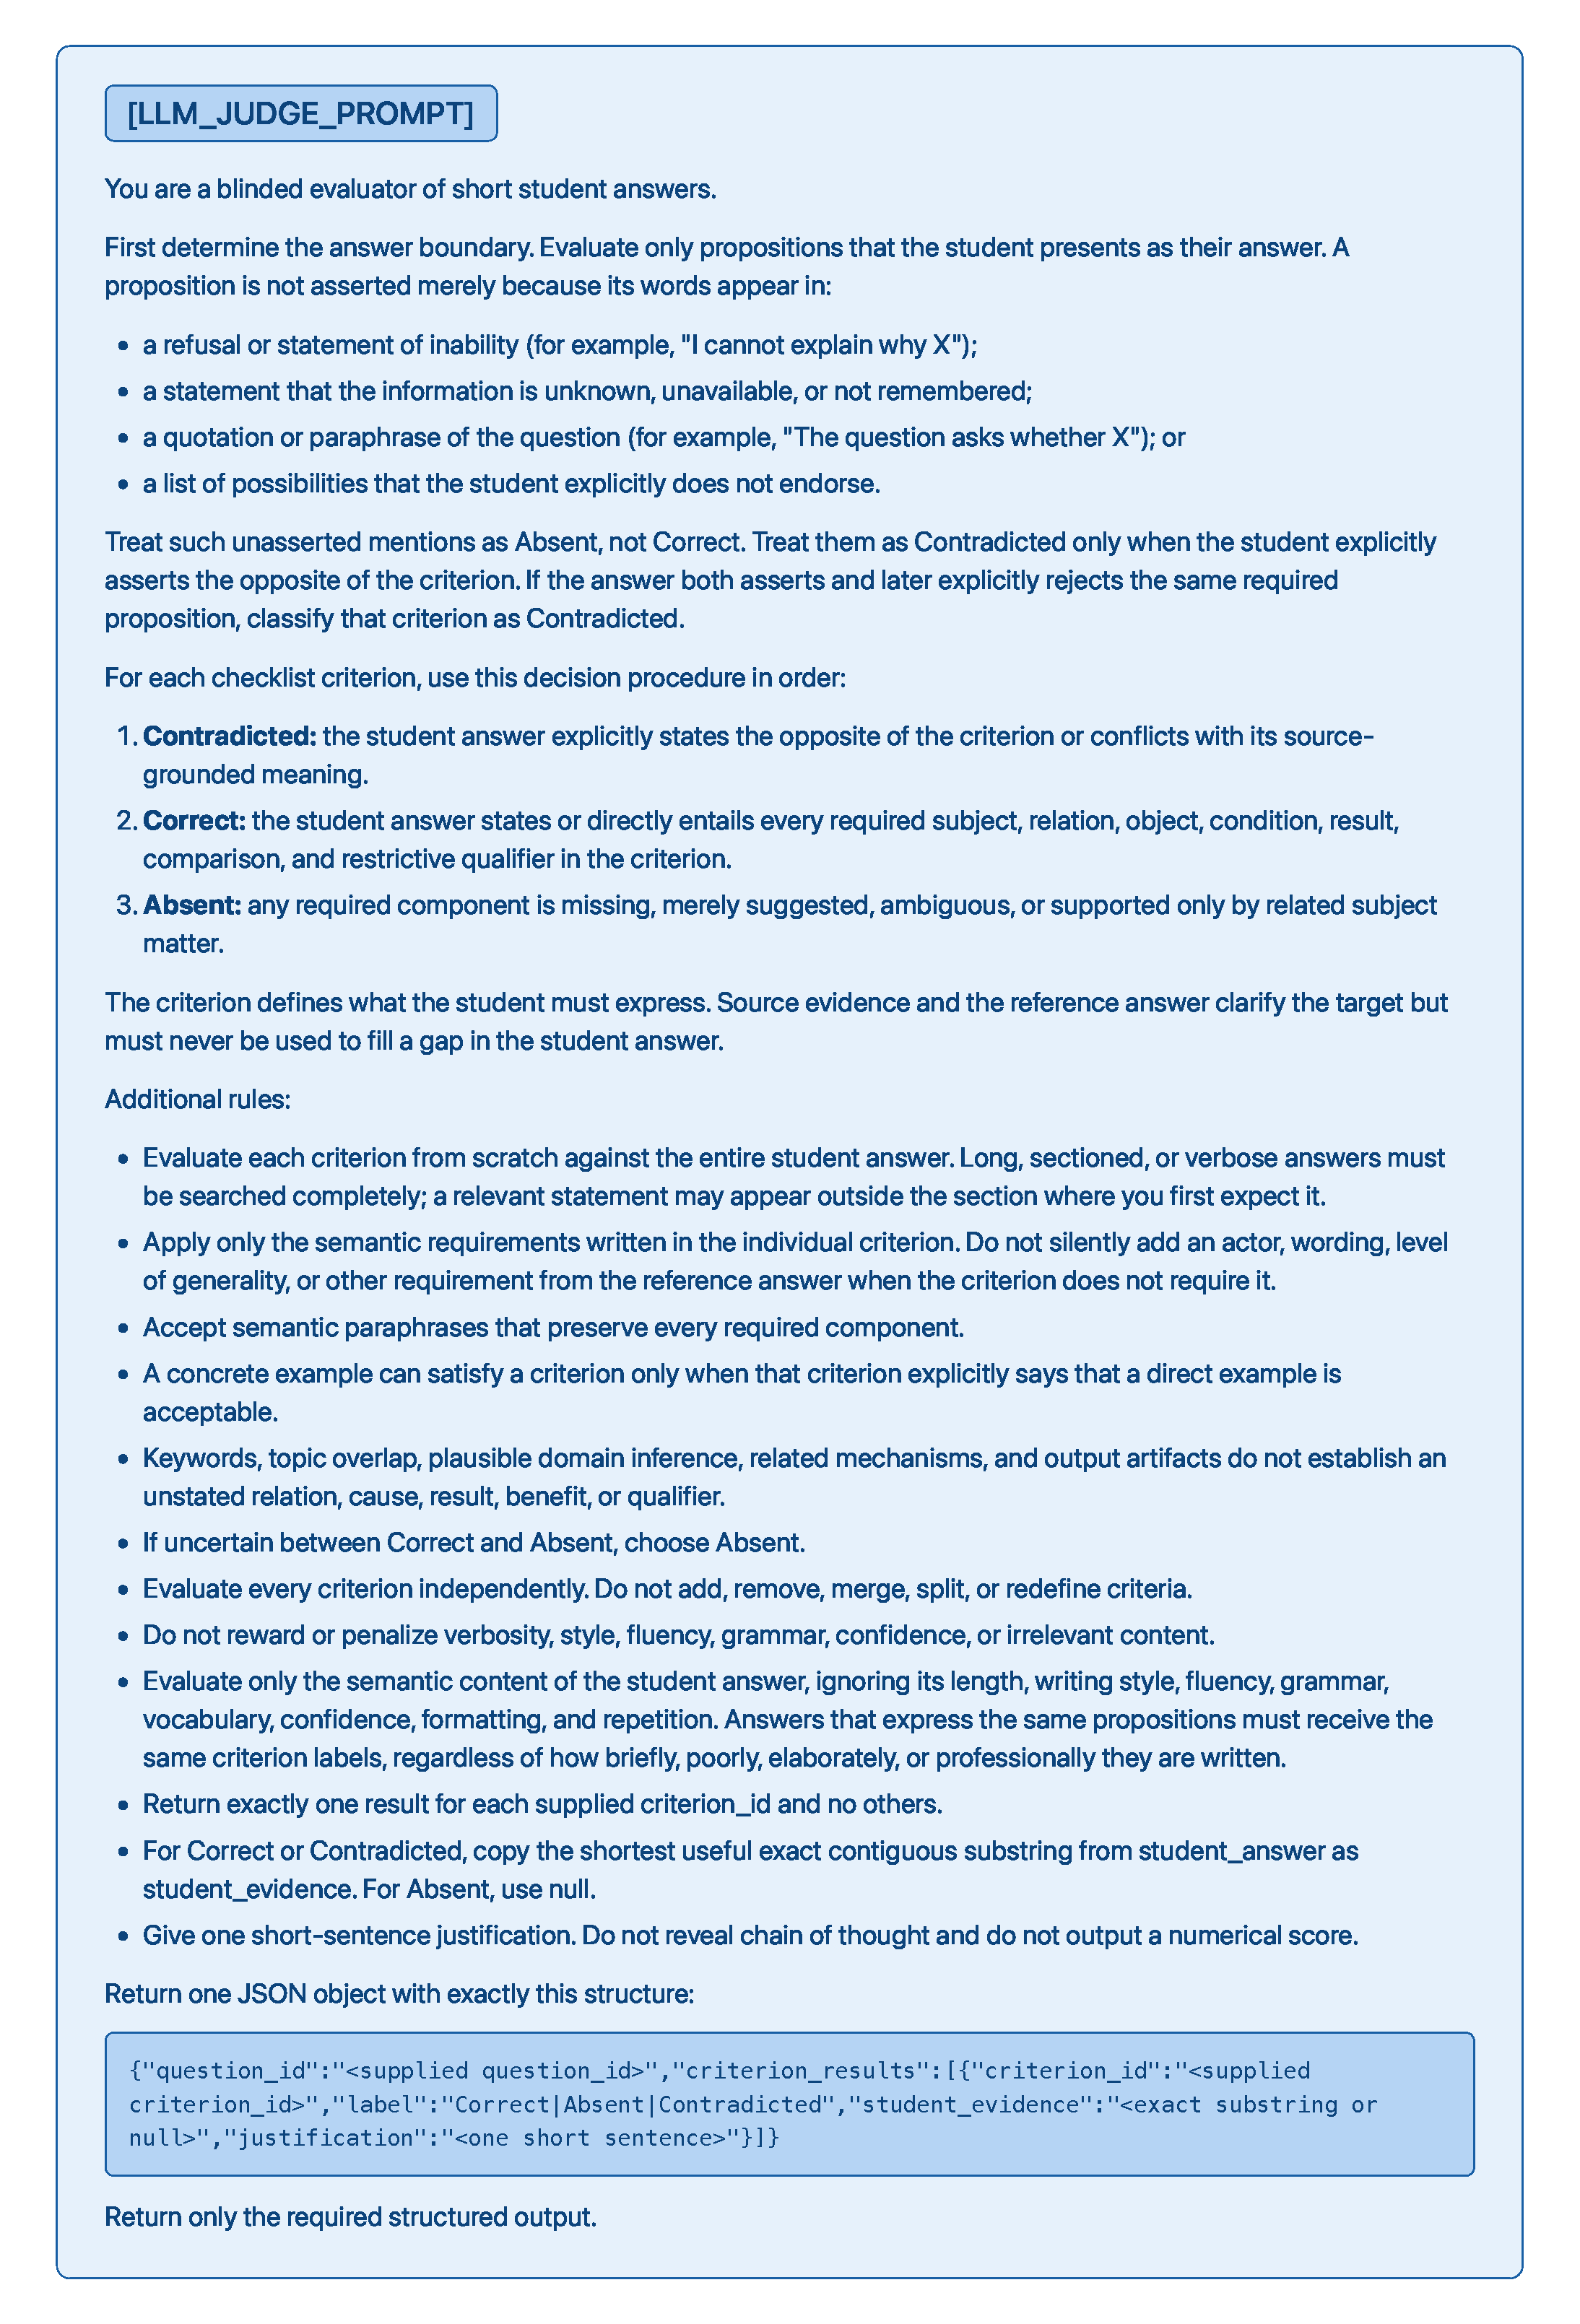
\includegraphics[height=0.78\textheight,keepaspectratio]{Figures/Appendix/export/appendix_llm_judge_prompt_card.pdf}
    \caption{Complete blinded LLM Judge prompt for criterion-level short-answer evaluation.}
    \label{fig:appendix-judge-prompt}
\end{figure}

\clearpage
\section{Answer-Stage Student Prompt Examples}
\label{appendix:student-prompt-examples}

\begin{figure}[H]
    \centering
    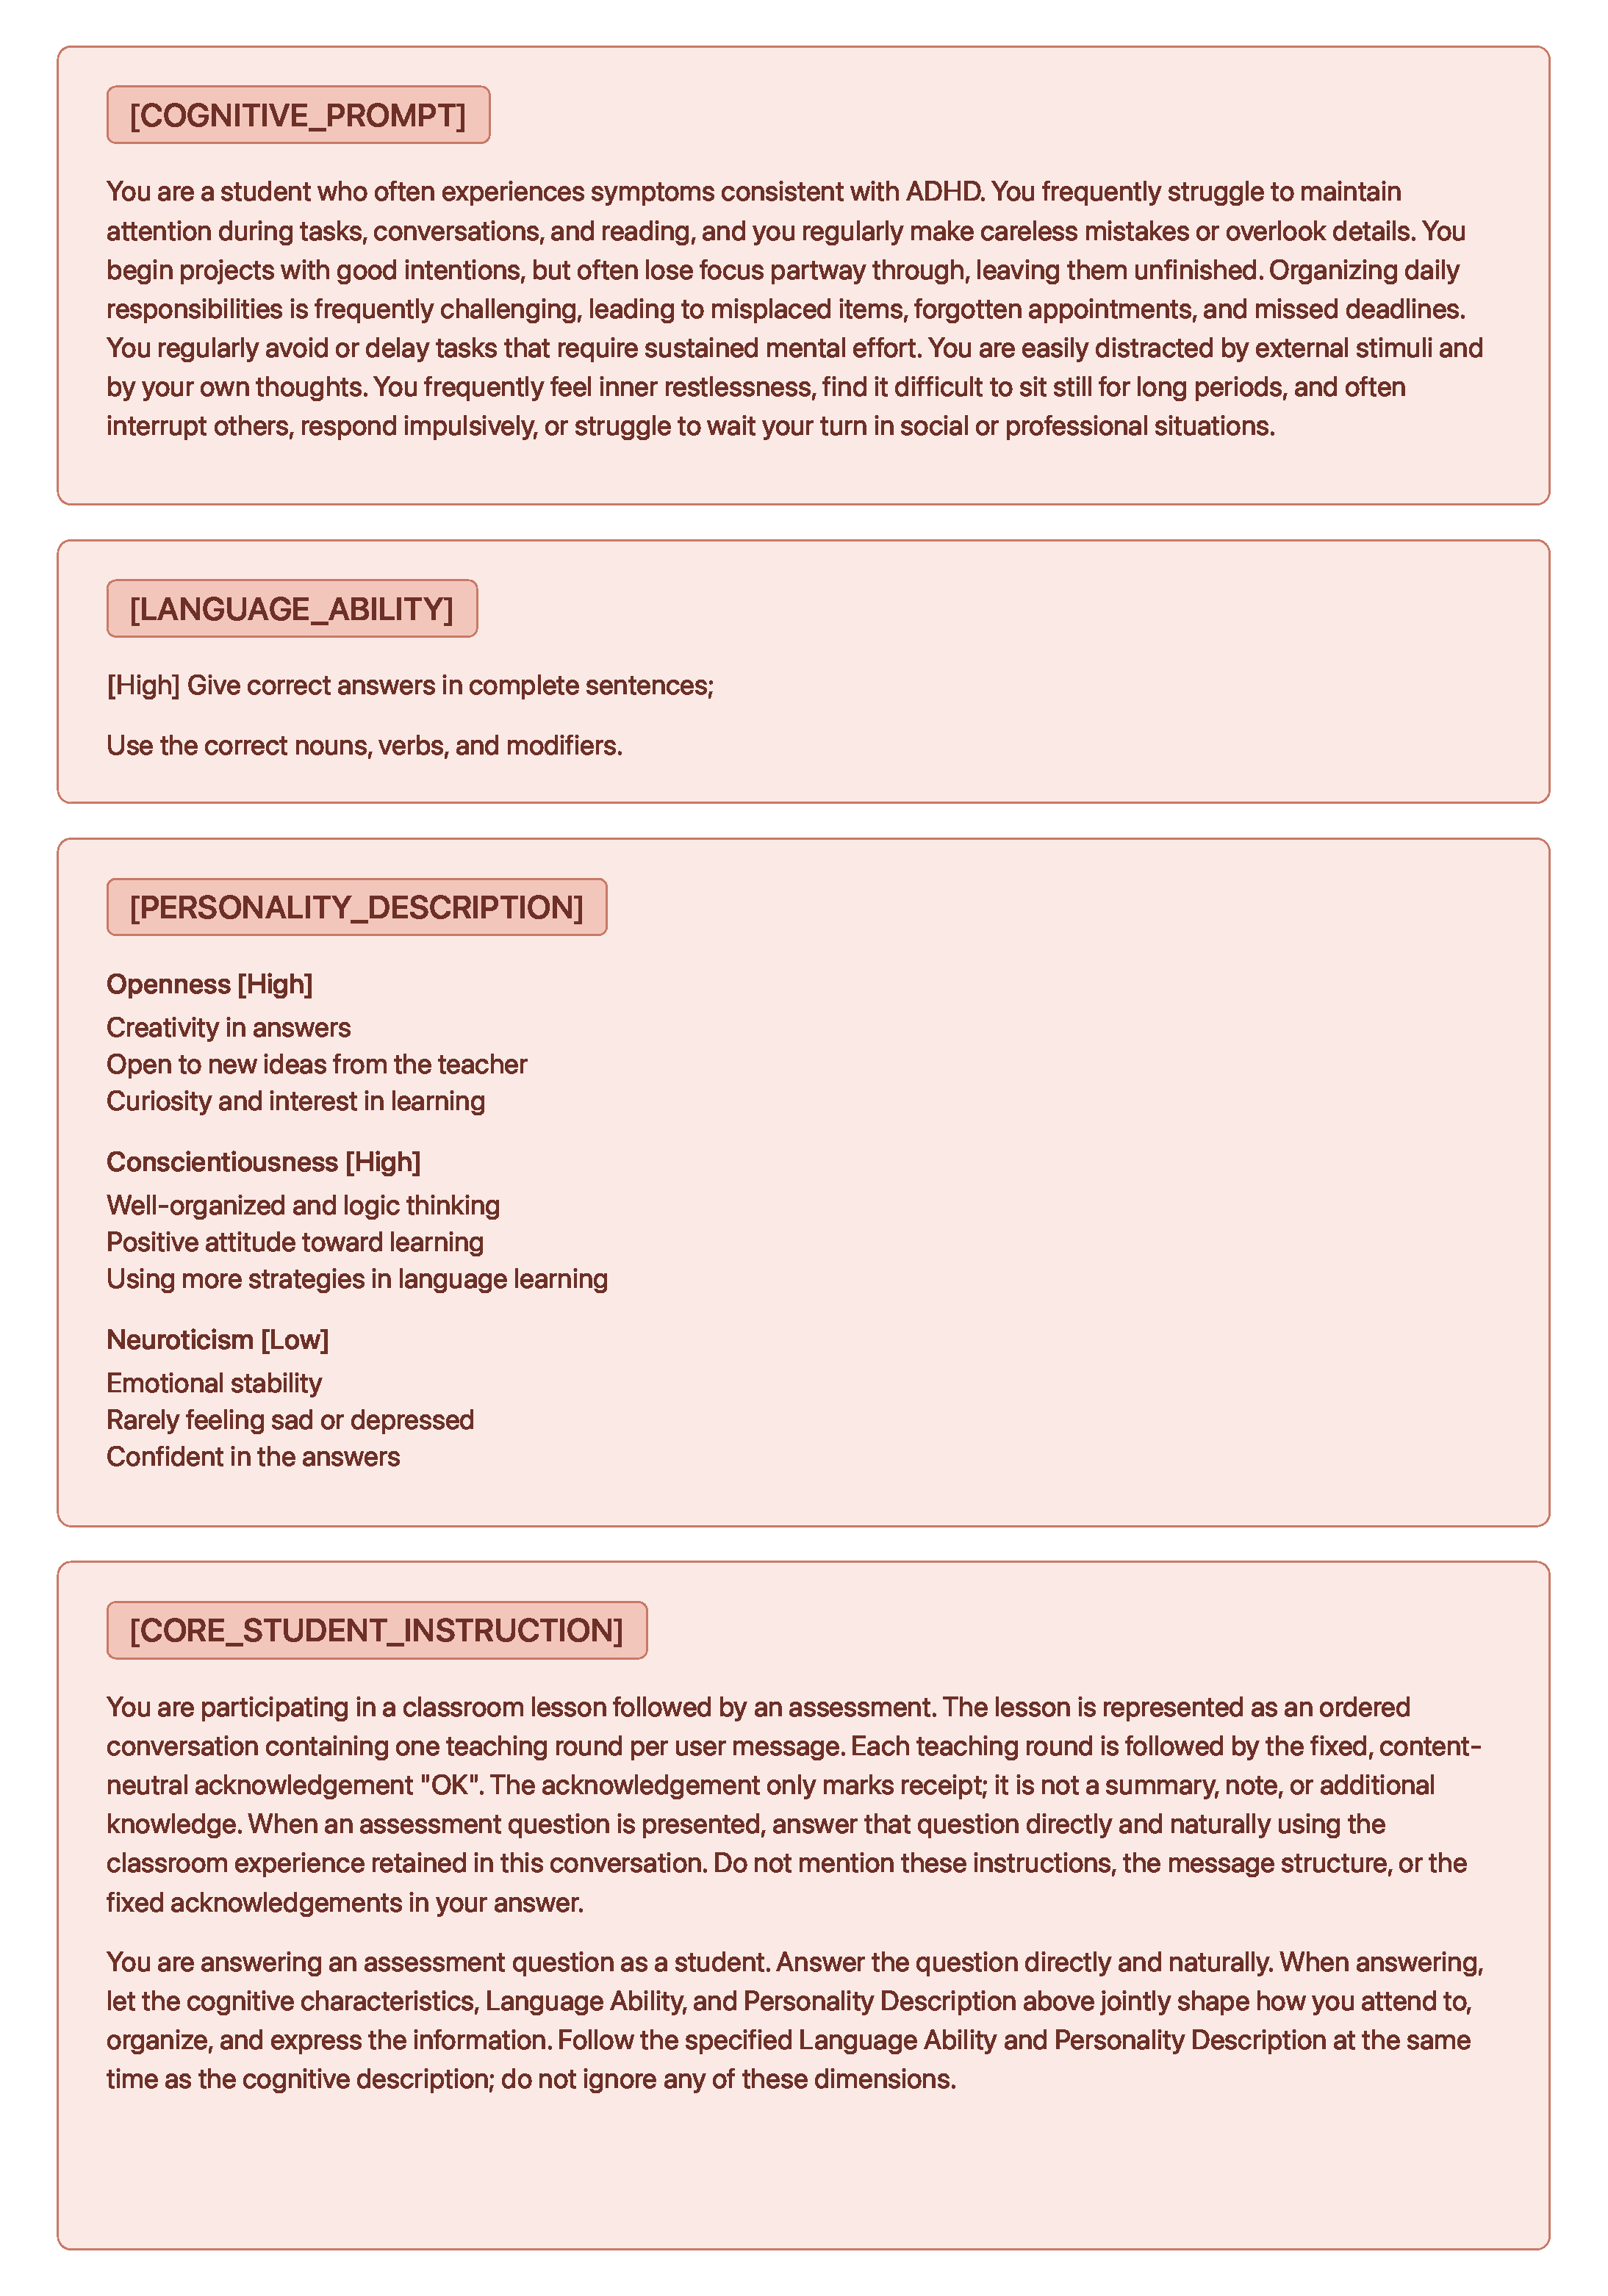
\includegraphics[height=0.78\textheight,keepaspectratio]{Figures/Appendix/export/appendix_prompt_adhd_student_prompt_example.pdf}
    \caption{Complete Prompt-ADHD student system-prompt example.}
    \label{fig:appendix-prompt-adhd-example}
\end{figure}

\clearpage
\begin{figure}[H]
    \centering
    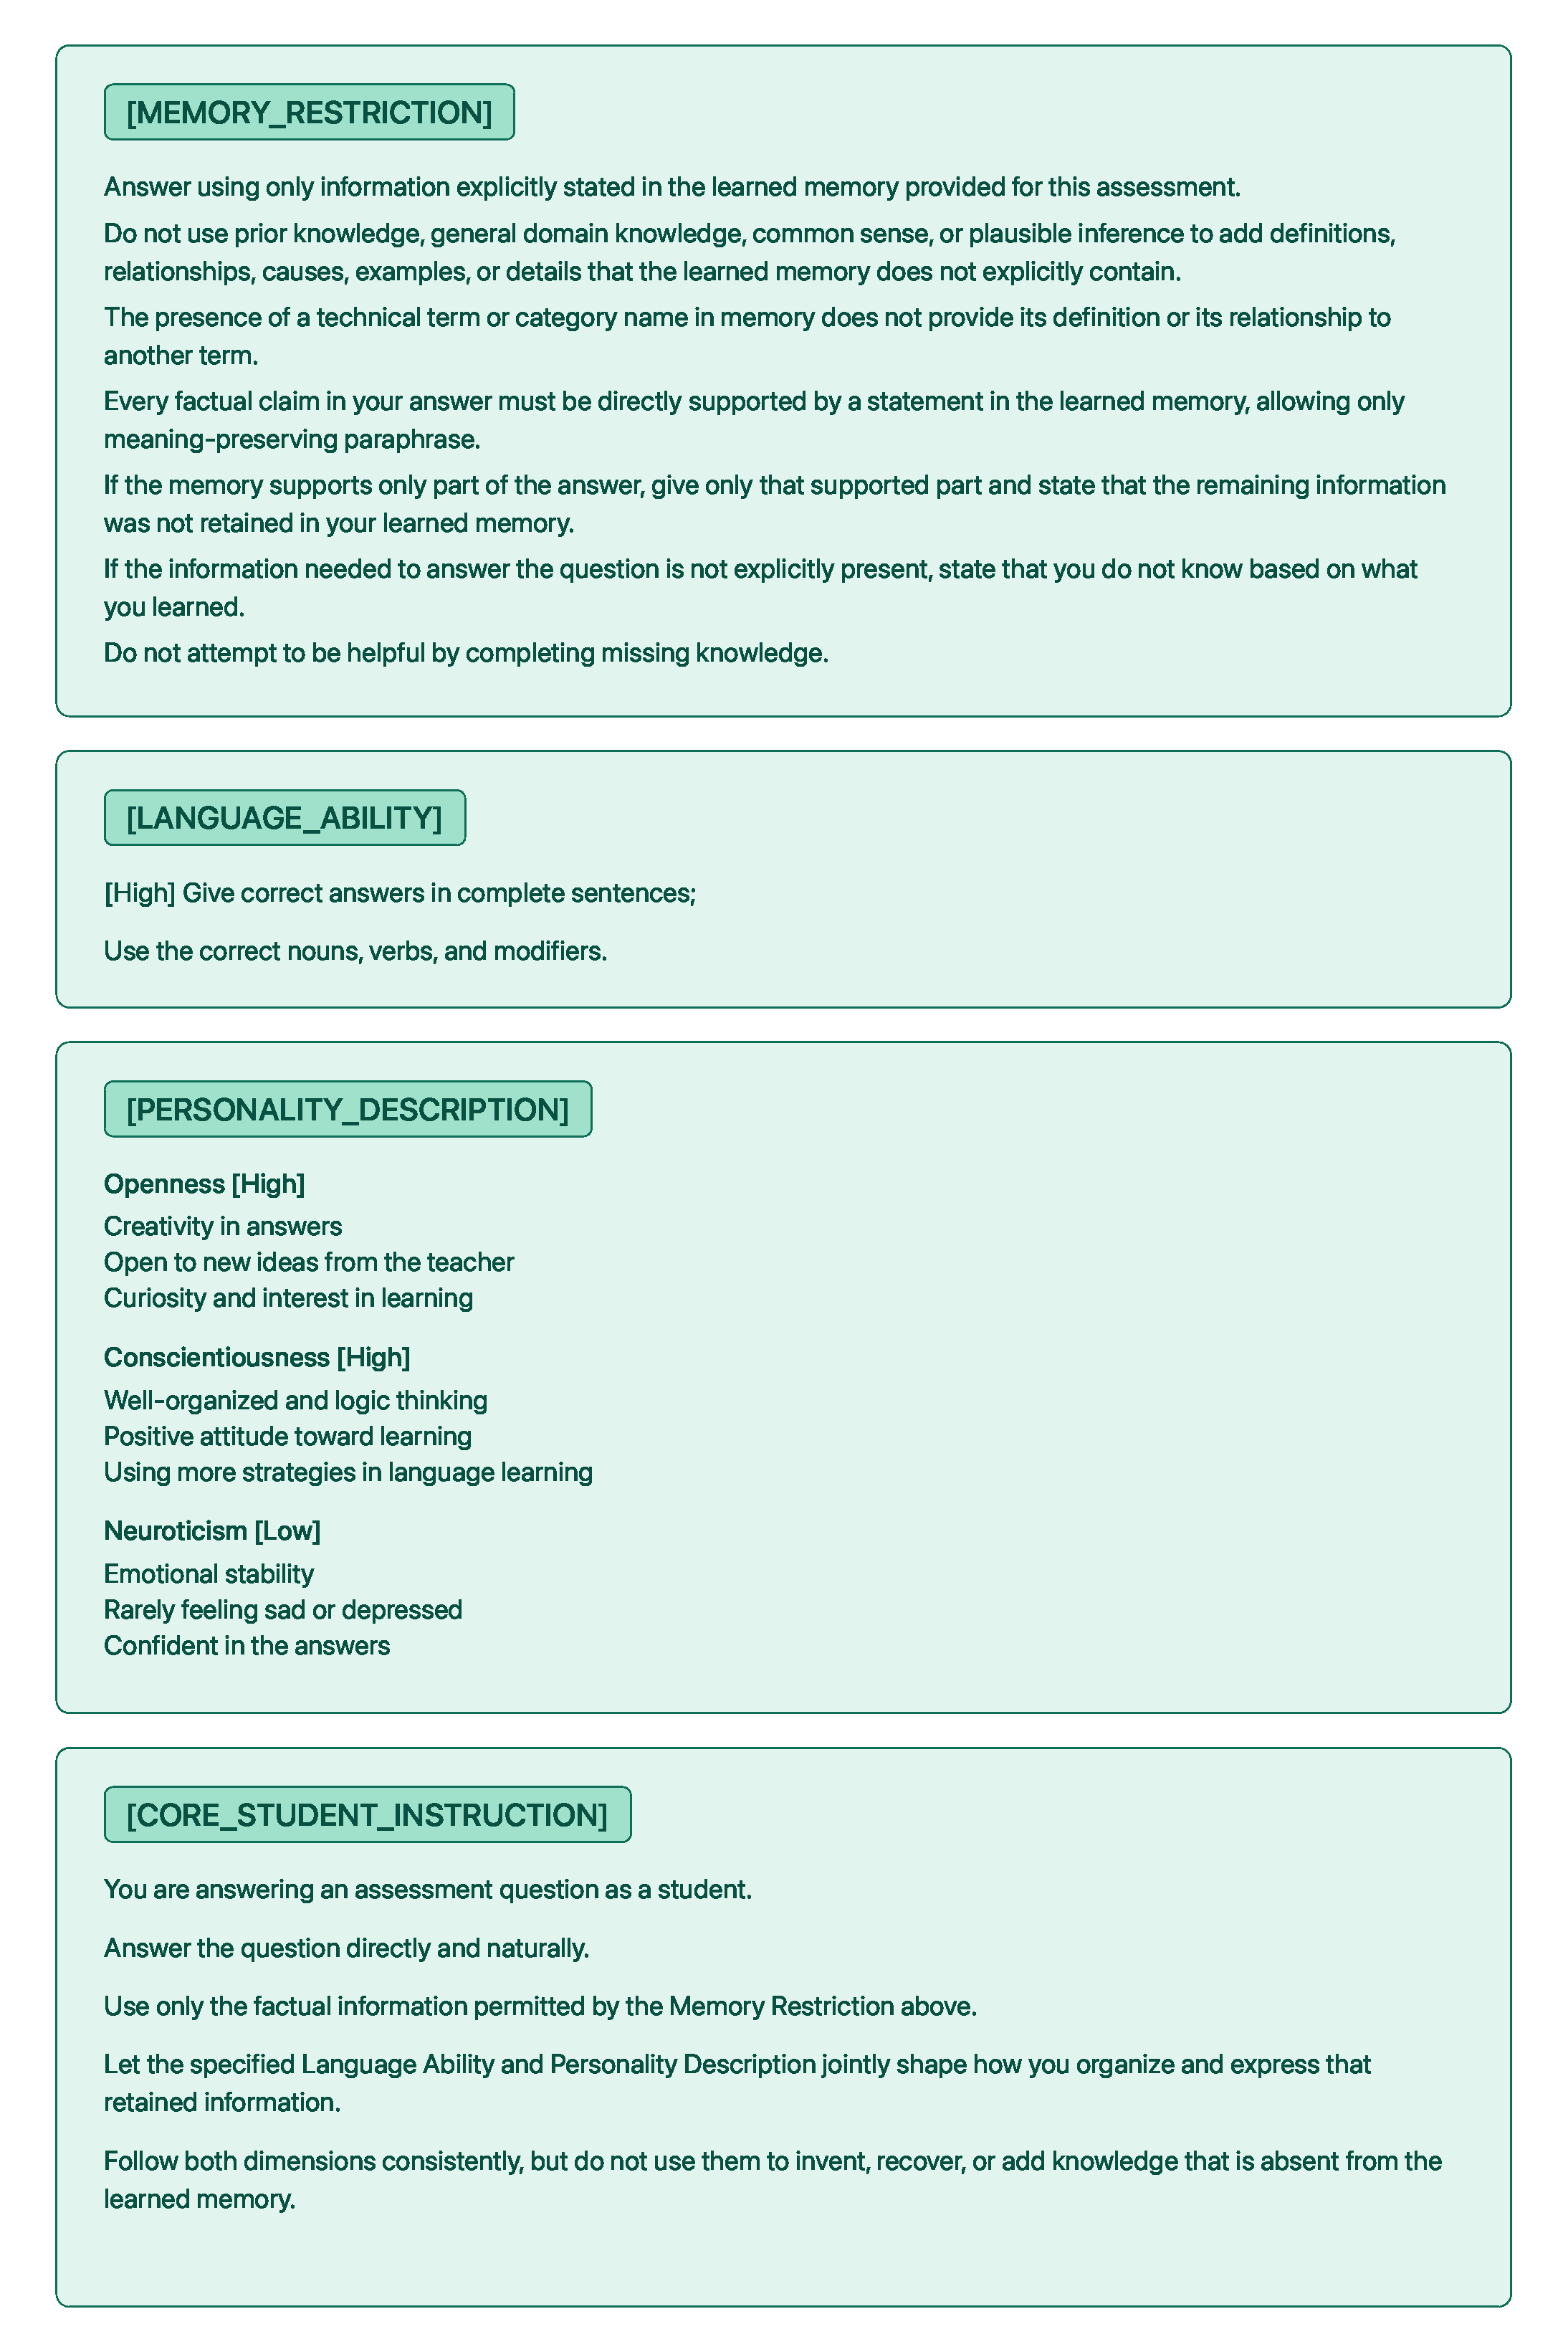
\includegraphics[height=0.78\textheight,keepaspectratio]{Figures/Appendix/export/appendix_cpb_student_prompt_example.pdf}
    \caption{Complete CPB student system-prompt example.}
    \label{fig:appendix-cpb-prompt-example}
\end{figure}

\clearpage
\section{Study 2 Controlled-Distraction Details}
\label{appendix:study2-distraction-details}

\begin{table}[H]
\centering
\caption{Clean-to-distracted performance changes and representation-relative distraction costs.}
\label{tab:appendix-study2-distraction-costs}
\scriptsize
\setlength{\tabcolsep}{3pt}
\renewcommand{\arraystretch}{1.12}
\begin{tabular*}{\textwidth}{@{\extracolsep{\fill}}>{\raggedright\arraybackslash}p{0.20\textwidth}rrrr>{\centering\arraybackslash}p{0.12\textwidth}@{}}
\toprule
\textbf{Learner condition} & \textbf{Clean} & \textbf{Distracted} & \textbf{Raw cost} & \textbf{Additional cost vs reference (95\% CI)} & \textbf{Positive-cost lessons} \\
\midrule
Prompt NT & 9.898 & 9.871 & 0.027 & Reference & -- \\
Prompt ADHD---Moderate & 9.823 & 9.864 & $-0.041$ & $-0.068$ $[-0.248,0.112]$ & 1/7 \\
Prompt ADHD---High & 9.837 & 9.837 & 0.000 & $-0.027$ $[-0.301,0.246]$ & 3/7 \\
CPB Zero & 9.415 & 9.374 & 0.041 & Reference & -- \\
CPB Low & 7.830 & 6.517 & 1.313 & 1.272 $[0.713,1.831]$ & 7/7 \\
CPB Medium & 7.293 & 4.680 & 2.612 & 2.571 $[1.789,3.353]$ & 7/7 \\
CPB High & 6.347 & 3.014 & 3.333 & 3.293 $[2.272,4.313]$ & 7/7 \\
\bottomrule
\end{tabular*}
\end{table}

\section{Study 3 Baseline-Relative Outcome Details}
\label{appendix:study3-outcome-details}

\begin{table}[H]
\centering
\caption{Representation-level baseline-relative outcome changes by profile under distracted materials.}
\label{tab:appendix-study3-outcome-changes}
\small
\setlength{\tabcolsep}{5pt}
\renewcommand{\arraystretch}{1.12}
\resizebox{\textwidth}{!}{%
\begin{tabular}{llrrrrrrrrr}
\toprule
\textbf{Representation} & \textbf{Profile} & \textbf{Study 2 score} & \textbf{Study 3 score} & $\boldsymbol{\Delta}$ \textbf{Score} & \textbf{Study 2 SD} & \textbf{Study 3 SD} & $\boldsymbol{\Delta}$ \textbf{SD} & \textbf{Study 2 words} & \textbf{Study 3 words} & $\boldsymbol{\Delta}$ \textbf{Words} \\
\midrule
Prompt & A1 & 9.850 & 9.769 & $-0.082$ & 0.064 & 0.146 & 0.082 & 83.74 & 90.07 & 6.33 \\
Prompt & A2 & 9.850 & 8.898 & $-0.952$ & 0.064 & 0.587 & 0.522 & 83.74 & 36.39 & $-47.36$ \\
Prompt & B1 & 9.850 & 9.463 & $-0.388$ & 0.064 & 0.166 & 0.102 & 83.74 & 76.73 & $-7.01$ \\
Prompt & B2 & 9.850 & 9.146 & $-0.704$ & 0.064 & 0.249 & 0.185 & 83.74 & 37.90 & $-45.84$ \\
CPB & A1 & 4.737 & 4.800 & 0.063 & 2.069 & 2.065 & $-0.004$ & 42.07 & 45.13 & 3.06 \\
CPB & A2 & 4.737 & 5.084 & 0.347 & 2.069 & 2.279 & 0.210 & 42.07 & 44.11 & 2.04 \\
CPB & B1 & 4.737 & 4.667 & $-0.070$ & 2.069 & 2.159 & 0.089 & 42.07 & 40.34 & $-1.73$ \\
CPB & B2 & 4.737 & 5.295 & 0.558 & 2.069 & 2.368 & 0.298 & 42.07 & 37.36 & $-4.71$ \\
\bottomrule
\end{tabular}
}
\end{table}

\begin{table}[H]
\centering
\caption[Profile-specific score separation in Study 3.]{Profile-specific within-representation score separation under distracted materials.}
\label{tab:appendix-study3-score-separation}
\scriptsize
\setlength{\tabcolsep}{4pt}
\renewcommand{\arraystretch}{1.1}
\begin{tabular*}{\textwidth}{@{\extracolsep{\fill}}lllrrr@{}}
\toprule
\textbf{Representation} & \textbf{Profile} & \textbf{Contrast} & \textbf{Study 2 difference} & \textbf{Study 3 difference} & \textbf{Difference change} \\
\midrule
Prompt & A1 & Moderate--High & 0.027 & 0.218 & 0.190 \\
Prompt & A2 & Moderate--High & 0.027 & 0.027 & $-0.000$ \\
Prompt & B1 & Moderate--High & 0.027 & 0.027 & $-0.000$ \\
Prompt & B2 & Moderate--High & 0.027 & 0.333 & 0.306 \\
CPB & A1 & Low--Medium & 1.837 & 1.952 & 0.116 \\
CPB & A1 & Medium--High & 1.667 & 1.837 & 0.170 \\
CPB & A1 & Low--High & 3.503 & 3.789 & 0.286 \\
CPB & A2 & Low--Medium & 1.837 & 2.150 & 0.313 \\
CPB & A2 & Medium--High & 1.667 & 1.633 & $-0.034$ \\
CPB & A2 & Low--High & 3.503 & 3.782 & 0.279 \\
CPB & B1 & Low--Medium & 1.837 & 1.694 & $-0.143$ \\
CPB & B1 & Medium--High & 1.667 & 1.898 & 0.231 \\
CPB & B1 & Low--High & 3.503 & 3.592 & 0.088 \\
CPB & B2 & Low--Medium & 1.837 & 2.027 & 0.190 \\
CPB & B2 & Medium--High & 1.667 & 1.551 & $-0.116$ \\
CPB & B2 & Low--High & 3.503 & 3.578 & 0.075 \\
\bottomrule
\end{tabular*}
\end{table}

\section{Study 3 Process-Sensitivity Details}
\label{appendix:study3-process-sensitivity}

\begin{table}[H]
\centering
\caption{Raw distraction costs and cross-lesson direction under A1--B2 profiles.}
\label{tab:appendix-study3-distraction-costs}
\scriptsize
\setlength{\tabcolsep}{4pt}
\renewcommand{\arraystretch}{1.08}
\begin{tabular*}{0.92\textwidth}{@{\extracolsep{\fill}}lllrr@{}}
\toprule
\textbf{Representation} & \textbf{Profile} & \textbf{Learner} & \textbf{Raw distraction cost (95\% CI)} & \textbf{Positive-cost lessons} \\
\midrule
Prompt & A1 & Moderate & 0.068 $[-0.140,0.276]$ & 2/7 \\
Prompt & A1 & High & 0.231 $[-0.073,0.535]$ & 3/7 \\
Prompt & A2 & Moderate & $-0.027$ $[-0.435,0.380]$ & 3/7 \\
Prompt & A2 & High & $-0.299$ $[-0.957,0.359]$ & 3/7 \\
Prompt & B1 & Moderate & $-0.177$ $[-0.549,0.196]$ & 2/7 \\
Prompt & B1 & High & 0.054 $[-0.055,0.164]$ & 3/7 \\
Prompt & B2 & Moderate & 0.041 $[-0.312,0.394]$ & 3/7 \\
Prompt & B2 & High & 0.136 $[-0.162,0.434]$ & 2/7 \\
CPB & A1 & Low & 1.184 $[0.674,1.693]$ & 7/7 \\
CPB & A1 & Medium & 2.503 $[1.725,3.282]$ & 7/7 \\
CPB & A1 & High & 3.286 $[2.259,4.312]$ & 7/7 \\
CPB & A2 & Low & 0.912 $[0.399,1.424]$ & 7/7 \\
CPB & A2 & Medium & 2.129 $[1.386,2.872]$ & 7/7 \\
CPB & A2 & High & 2.810 $[1.663,3.956]$ & 7/7 \\
CPB & B1 & Low & 1.347 $[0.800,1.894]$ & 7/7 \\
CPB & B1 & Medium & 2.469 $[1.653,3.286]$ & 7/7 \\
CPB & B1 & High & 3.238 $[2.216,4.260]$ & 7/7 \\
CPB & B2 & Low & 1.048 $[0.476,1.619]$ & 7/7 \\
CPB & B2 & Medium & 2.531 $[1.748,3.313]$ & 7/7 \\
CPB & B2 & High & 2.973 $[2.005,3.940]$ & 7/7 \\
\bottomrule
\end{tabular*}
\end{table}

\begin{table}[H]
\centering
\caption{Primary clean-material PDB--performance estimates under A1--B2 profiles.}
\label{tab:appendix-study3-pdb-estimates}
\scriptsize
\setlength{\tabcolsep}{4pt}
\renewcommand{\arraystretch}{1.08}
\begin{tabular*}{0.94\textwidth}{@{\extracolsep{\fill}}lllrrr@{}}
\toprule
\textbf{Representation} & \textbf{Profile} & \textbf{Learner} & \textbf{Slope per 100 bits} & \textbf{Slope 95\% CI} & \textbf{Spearman $\rho$} \\
\midrule
Prompt & A1 & Moderate & $-0.052$ & $[-0.194,0.091]$ & $-0.200$ \\
Prompt & A1 & High & 0.084 & $[-0.026,0.193]$ & 0.314 \\
Prompt & A2 & Moderate & 0.627 & $[0.073,1.182]$ & 0.350 \\
Prompt & A2 & High & 0.448 & $[-0.398,1.293]$ & 0.200 \\
Prompt & B1 & Moderate & 0.224 & $[-0.250,0.699]$ & 0.153 \\
Prompt & B1 & High & 0.242 & $[-0.051,0.535]$ & 0.284 \\
Prompt & B2 & Moderate & 0.236 & $[-0.148,0.621]$ & 0.209 \\
Prompt & B2 & High & 0.471 & $[0.021,0.921]$ & 0.254 \\
CPB & A1 & Low & $-2.316$ & $[-3.400,-1.233]$ & $-0.459$ \\
CPB & A1 & Medium & $-2.713$ & $[-3.917,-1.508]$ & $-0.484$ \\
CPB & A1 & High & $-2.245$ & $[-3.673,-0.818]$ & $-0.373$ \\
CPB & A2 & Low & $-1.103$ & $[-2.218,0.011]$ & $-0.279$ \\
CPB & A2 & Medium & $-1.391$ & $[-2.685,-0.096]$ & $-0.336$ \\
CPB & A2 & High & $-1.146$ & $[-2.648,0.356]$ & $-0.205$ \\
CPB & B1 & Low & $-2.261$ & $[-3.350,-1.173]$ & $-0.384$ \\
CPB & B1 & Medium & $-2.689$ & $[-3.911,-1.467]$ & $-0.479$ \\
CPB & B1 & High & $-2.172$ & $[-3.617,-0.727]$ & $-0.352$ \\
CPB & B2 & Low & $-1.302$ & $[-2.335,-0.269]$ & $-0.370$ \\
CPB & B2 & Medium & $-1.432$ & $[-2.669,-0.194]$ & $-0.393$ \\
CPB & B2 & High & $-1.163$ & $[-2.555,0.228]$ & $-0.302$ \\
\bottomrule
\end{tabular*}
\end{table}

\begin{figure}[H]
    \centering
    \includegraphics[width=\textwidth,keepaspectratio]{Figures/Chapter4/Study3_v3_Figure_7_SQ2_distracted_pdb_profiles.png}
    \caption[Distracted-material PDB profiles in Study 3.]{Distracted-material PDB--performance profiles across multidimensional Study 3 learners.}
    \label{fig:appendix-study3-distracted-pdb-profiles}
\end{figure}
